\epigraph{An undefined term is the beginning of every definition}
{\textit{Bertrand Russell}}

Throughout this guide, a number of links, terms, and abbreviations come up repeatedly, which are now collated here for reference. 

\textbf{\href{https://www.southampton.ac.uk/studentservices/index.page}{The Student Hub}} \\
24/7, first point of contact support service for students providing advice and guidance on things like wellbeing, finance, accommodation, etc. 

\textbf{\href{https://sotonac.sharepoint.com/}{SUSSED}} \\
The University's main intranet portal used by students and staff for news, updates, events, and quick links to key services. 

\textbf{\href{https://www.southampton.ac.uk/about/faculties-schools-departments/school-of-mathematical-sciences}{School of Mathematical Sciences}} 

\textbf{\href{https://www.southampton.ac.uk/studentadmin/academic-support-guidance/personal-tutor.page}{PAT}} - Personal Academic Tutor \\  
A member of staff who will help you settle in your studies, support your academic progress and act as a key contact for queries, or direct you to other support services if you need it. 

\textbf{Office Hours}\\
Designated times when lecturers are available for students to drop by to discuss academic content, feedback, or module-related questions outside of scheduled lectures. 

\textbf{\href{https://library.soton.ac.uk/feedback/types}{Formative and Summative Assessments}}\\
Formative mark doesn’t to count towards your final mark for the module; summative counts towards the final mark.

\textbf{Accreditations} \\
Actuarial science programmes at the University of Southampton are accredited by the \textbf{\href{https://actuaries.org.uk/}{Institute and Faculty of Actuaries (IFoA)}}, allowing students to gain exemptions from core principles examinations (CS1, CS2, CM1, CM2, CB1, CB2). Key accredited programs include BSc Mathematics with Actuarial Science and BSc Economics and Actuarial Science. For further details, contact Actuarial Sciences course lead. 

\textbf{\href{https://www.southampton.ac.uk/about/governance/regulations-policies/taught-students/general/credit-accumulation-transfer}{CATS/ECATS}}\\
Systems used to measure and transfer academic credit for modules and degrees.

\textbf{\href{https://www.southampton.ac.uk/quality/governance/sslctaught.page}{SSLC}} - Student Staff Liaison Committee \\
Meeting where student representatives and academic staff discuss and resolve issues, enhancing the overall education and student experience

\textbf{\href{https://www.susu.org/representation/academic-representation.html}{Course and Academic Reps}} \\
Students volunteers who collect feedback on teaching, learning, and assessments to improve the student experience and liaise with staff in SSLCs. 

\textbf{\href{https://www.susu.org/}{SUSU}} - Southampton University Student Union \\
A student-led organisation independent from the university that is run by students, for students. 

\textbf{\href{https://www.susu.org/groups/sums}{SUMS}} - Southampton University Maths Society 

\textbf{\href{https://www.susu.org/groups/suas}{SUAS}} - Southampton University Actuarial Society 

\textbf{\href{https://www.southampton.ac.uk/library/index.page}{Library Services}}
 
\textbf{\href{https://library.soton.ac.uk/sash}{Library - Academic Skills Service}}

\textbf{\href{https://www.southampton.ac.uk/student-life/accommodation}{Student Accommodation}}

\textbf{\href{https://store.southampton.ac.uk/short-courses/halls/student-experience-engagement/kitchen-school}{Kitchen School}} \\
A hands-on, expert-led cookery program for students designed to teach basic culinary skills, healthy cooking, and food safety. 

\begin{figure}[H]
    \centering
    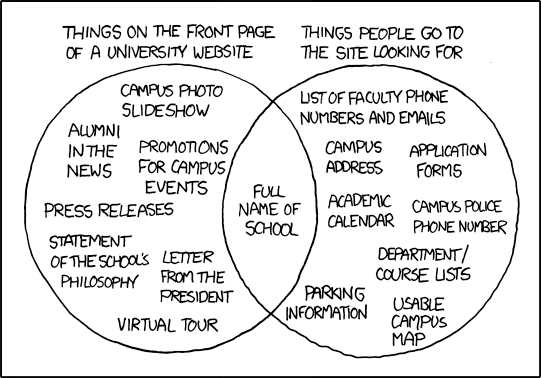
\includegraphics[width=0.6\linewidth]{xkcd/uniWebsite.png}
    \caption{\textbf{\href{https://xkcd.com/773/}{University Website}}}
\end{figure}

\begin{figure}[H]
    \centering
    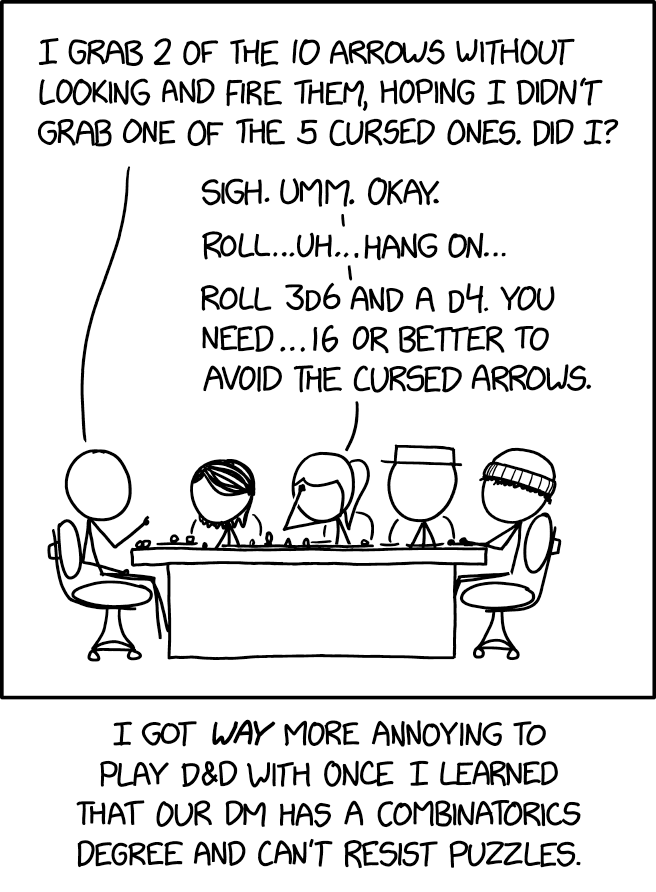
\includegraphics[width=0.5\linewidth]{xkcd/dnd.png}
    \caption{\textbf{\href{https://xkcd.com/3015/}{DnD Combinatorics}}}
\end{figure}
